\documentclass[11pt,letterpaper]{article}
\usepackage[lmargin=1in,rmargin=1in,tmargin=1in,bmargin=1in]{geometry}
\usepackage{../style/homework}
\usepackage{../style/commands}
\setbool{quotetype}{false} % True: Side; False: Under
\setbool{hideans}{true} % Student: True; Instructor: False

% -------------------
% Content
% -------------------
\begin{document}

\homework{15: Due 12/08}{Nothing goes over my head. My reflexes are too fast. I would catch it.}{Drax, Guardians of the Galaxy}

% Problem 1
\problem{10} Find and plot the solution to the system of equations given in the graph below:
	\[
	\fbox{
	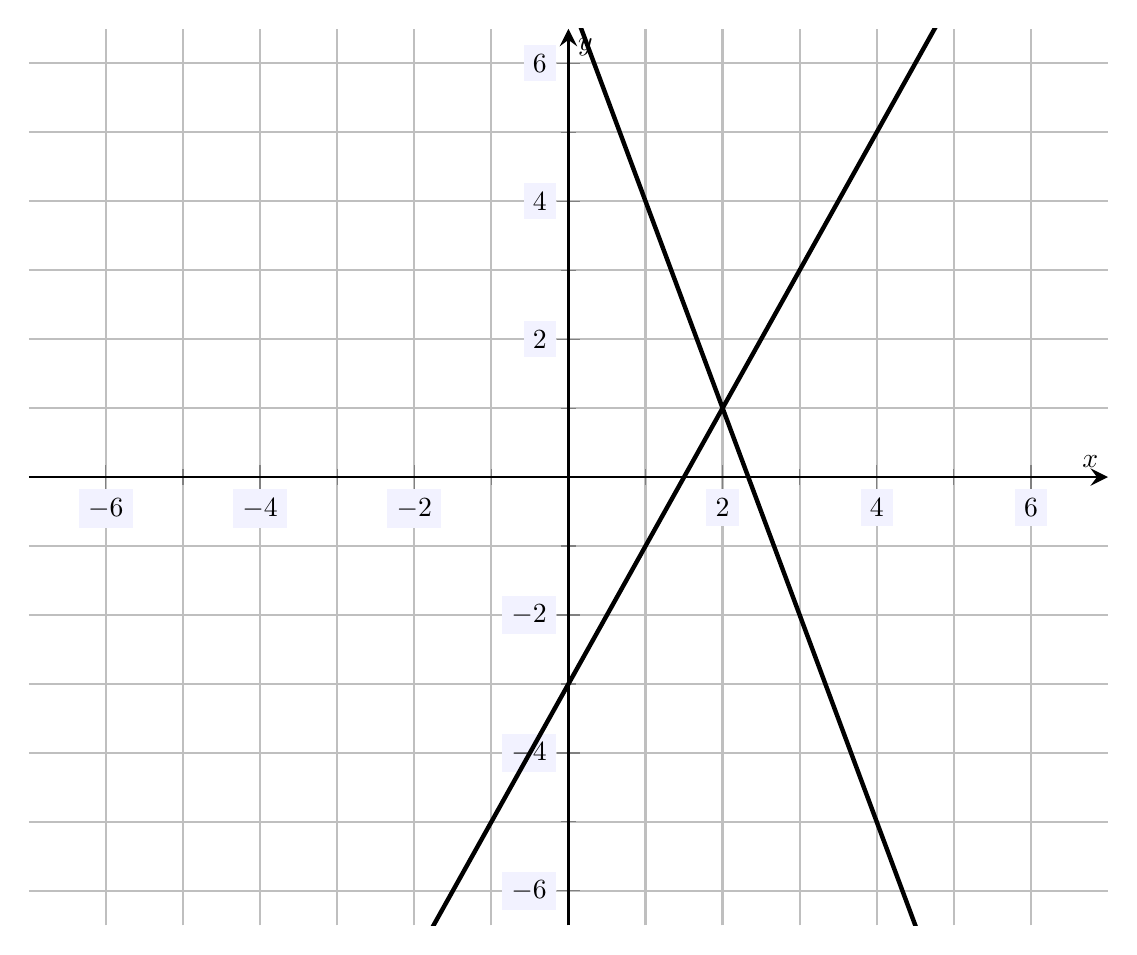
\begin{tikzpicture}[scale=2,every node/.style={scale=0.5}]
	\begin{axis}[
	grid=both,
	axis lines=middle,
	ticklabel style={fill=blue!5!white},
	xmin= -7, xmax=7,
	ymin= -6.5, ymax=6.5,
	xtick={-6,-4,-2,0,2,4,6},
	ytick={-6,-4,-2,0,2,4,6},
	minor tick = {-5,-3,...,5},
	xlabel=\(x\),ylabel=\(y\),
	]
	\addplot[thick, domain= -7:7,samples=150] {7 - 3*x};
	\addplot[thick, domain= -7:7,samples=150] {2*x - 3};
	\end{axis}
	\end{tikzpicture}
	}
	\] \pspace





\newpage





% Problem 2
\problem{10} Show that $(1, -2)$ is the solution to the system of equations below.
	\[
	\begin{aligned}
	-5x + 3y&= -11 \\
	3x - 5y&= 13
	\end{aligned}
	\]





\newpage





% Problem 3
\problem{10} Determine if the system of equations below has a solution. If not, explain why; if so, find the solution.
	\[
	\begin{aligned}
	4x - 3y&= -7 \\
	2x + 4y&= 13
	\end{aligned}
	\]





\newpage





% Problem 4
\problem{10} Determine if the system of equations below has a solution. If not, explain why; if so, find the solution. 
	\[
	\begin{aligned}
	10x - 4y&= 12 \\
	-5x + 2y&= 4
	\end{aligned}
	\]


%\printpoints
\end{document}